\documentclass[12pt]{article}
\title{\textsc {RSA Cryptosystem}}
\author{Luke Pereira - 2017 }
\date{}
\usepackage[margin=1.7cm]{geometry}
\usepackage{dcs}
\usepackage{multicol}
\usepackage{amsmath}
\usepackage{graphicx}
\setlength\columnsep{15pt} 
\newcommand{\Mod}[1]{\ (\text{mod}\ #1)}

\begin{document}

\maketitle
\section*{History of Cryptography}
\begin{multicols}{2}

The word cryptography, derived from the Greek words krypt\'{o}s, meaning "hidden", and graphein, meaning "writing", can broadly be understood as such - it is the practice of hiding the meaning or content of communications. More precisely, an encrypted message is typically made to be indistinguishable from random noise in an effort to prevent a third party adversary or the general public from ascertaining any useful information from the original private message.

In 1883, the Dutch cryptographer Auguste Kerckhoffs formulated six design axioms for military ciphers. They are now known as Kerckhoffs' principles [1] and are expressed as follows:
\begin{enumerate}
\itemsep-0.4em 
    \item The system must be practically, if not mathematically, indecipherable;
    \item It should not require secrecy, and it should not be a problem if it falls into enemy hands;
    \item It must be possible to communicate and remember the key without using written notes, and correspondents must be able to change or modify it at will;
    \item It must be applicable to telegraph communications;
    \item It must be portable, and should not require several persons to handle or operate;
    \item Lastly, the system must be easy to use and should not be stressful  or require its users to know and comply with a long list of rules.
\end{enumerate}

The second principle has proven to be particularly important in modern cryptosystems and their use of secret keys. It expresses the notion that despite an attacker's access to or familiarity with a cryptosystem, it is critical that they are still unable to determine a given message without solving for a computationally infeasible problem. 

A cryptosystem can be more rigorously described with the following sets and functions [2]:
\renewcommand\labelitemi{\tiny$\bullet$}
\begin{itemize}
\itemsep0em 
\item $\Sigma$: The alphabet 

     i.e. $\Sigma=\{a,...,Z,0,...,9\}$ or $\Sigma=\{0,1\}$

\item $M \subseteq \Sigma^*$: the message space

\item $C \subseteq \Sigma^*$: the cyphertext space

\item $K$: the keyspace

\item $\forall e \in K, E_e(x):M \to C$ 
    
    $E_e(x)$ is a bijective encryption function

\item $\forall d \in K, D_d(x):C\to M$ 

    $D_d(x)$ is a bijective decryption function

\item $ \forall e \in K, \exists d \in K$ such that $D_d=E_e^{-1}$ 

    That is, $\forall m \in M, D_d(E_e(m))=m$

\end{itemize}

The proliferation of computers and communications systems has inspired an urgent demand to protect information in digital forms from an increasingly computationally powerful adversary. A groundbreaking development came in 1976 with the work of Diffie and Hellman [3] and their revolutionary concept of "public-key cryptography" and an ingenious method for a key exchange, the security of which relies on the infeasibility of the discrete logarithm problem. Then in 1978, Rivest, Shamir, and Adleman discovered the first complete public-key encryption and signature scheme, now known as RSA [4]. The RSA algorithm also relies on a mathematically hard problem, the infeasibility of factoring large integers. 

\maketitle
\section*{Diffie and Helman: \\ \large `New Directions in Cryptography'}

The conceptualization of the public-key cryptosystem, briefly described above, laid the foundation for the development of the RSA method. The 1978 paper directly motivated the RSA research, since Diffie and Helman had presented the idea but did not formulate any practical implementation of a concrete system.

In particular, Diffie and Hellman introduced the concept of "trap-door one-way" functions $E$ and $D$, to be used for encryption and decryption,  but did not present any examples. These functions are considered “one-way” because they are easy to compute in one direction but are very difficult to compute in the other direction. They are referred to as “trapdoor” functions because the inverse functions are in fact easy to compute after certain secret “trap-door” information is known.
 
\maketitle
\section*{The RSA Method}

Suppose that we have A and B (also known as Alice and Bob) who are two users of a public-key cryptosystem.
\begin{verbatim}
        (unsecured channel)
  Alice -----+-----+------- Bob
             |     |
             |     |
             |    Mallory 
             |    (malicious attacker)
            Eve 
           (eavesdropper)
         
\end{verbatim}
Alice creates a public and private key pair $(k_e, k_d)$ which have the feature that knowing one does not easily lead to knowing the other. Alice publishes her public key $k_e$ and keeps her private key securely hidden. $k_e$ and $k_d$ are inverses with respect to the $RSA(key, message)$ function, that is 

$$\text{RSA}(k_d, \text{RSA}(k_e, m))$$
\begin{center}
$= \text{RSA}(k_e, \text{RSA}(k_d, m))$

$=m \qquad \qquad \qquad \quad \quad \ $ 
\end{center}

To compute these public and private keys, 

\renewcommand\labelitemi{\tiny$\bullet$}
\begin{itemize}

\item Alice chooses two large primes, $p,q \in \mathbb{Z}$ and some value $e \in \mathbb{Z}$ which is relatively prime to $(p-1)(q-1)$. 

\item Next, Alice finds a natural number $d$ such that $e\cdot d \equiv 1 \mod{(p-1)(q-1)}$.

\item Alice now has private key $(pq,d)$ and public key $(pq,e)$.
\end{itemize}

To encrypt/decrypt a shared message,

\renewcommand\labelitemi{\tiny$\bullet$}
\begin{itemize}

\item Suppose Bob has a message $M \in \mathbb{N}$ and wants to encrypt and send it to Alice. 

\item Bob computes $ C \equiv M ^ e \pmod{pq}$ and sends the encrypted message C to Alice.

\item Alice computes $M \equiv C^d \pmod{pq}$, Bob's decrypted message.

\end{itemize}

\maketitle
\section*{Theorems and Identities}

The proof of correctness provided in the RSA paper relies on Fermat's Little Theorem, which states that if $p$ is prime and $p$ does not divide an integer $a$ then, $$ a^{p-1} \equiv 1 \Mod{p}$$
and an identity from Euler's theorem, which states that if $n$ and $M$ (a message in our case) are coprime positive integers, then 
\begin{equation} \label{eq:1}
M ^{\varphi(n)} \equiv 1 \Mod{n}  
\end{equation}
where $\varphi(n)$ is Euler's Totient function. $\varphi(n)$ gives the number of positive integers less than $n$ which are relatively prime to $n$. 
The following properties of the Euler totient function are applied: 

for prime numbers $p$,
$$\varphi(p) = p-1 $$ 

and if $n = pq$, then 
\begin{align} 
\varphi(n) &= \varphi(p) \cdot \varphi(q) \nonumber\\
&= (p-1)\cdot(q-1) \\ \label{eq2}
&= n - (p+q) +1 \nonumber
\end{align}

Also, since $d$ is relatively prime to $\varphi(n)$, it must have a multiplicative inverse $e$ such that
\begin{equation} \label{eq:3}
e\cdot d \equiv 1 \Mod{\varphi(n)} 
\end{equation}

\maketitle
\section*{Proof Of Correctness}
\begin{proof}
Recall that the encryption and decryption algorithms E and D for a message M and a cyphertext C are:

\begin{align}
C \equiv E(M) &\equiv M^e \pmod{n}, \nonumber\\
D(C) &\equiv C^d \pmod{n}. \nonumber
\end{align}

We can prove that deciphering works correctly if $e$ and $d$ are chosen as shown previously, by proving that the following equations hold:
\begin{equation} \label{eq:4}
D(E(M) = M.
\end{equation}
\begin{equation} \label{eq:5}
E(D(M) = M. 
\end{equation}

So,
\begin{align*}
D(E(M) \equiv (E(M))^d &\equiv (M^e)^d\Mod {n} \\
&=M^{e\cdot d} \Mod{n} \\
E(D(M)) \equiv (D(M))^e &\equiv (M^d)^e\Mod {n} \\
&=M^{e\cdot d} \Mod{n}
\end{align*}

We know that $M^{e\cdot d} $ can equivalently be expressed as $M^{k\cdot\varphi(n)+1}\Mod{n}$ for some $k\in \mathbb{Z}$. 
From $(1)$, we see that for all $M$ such that $p$ does not divide $M$,
$$M^{p-1} \equiv 1 \Mod{p} $$
and since $(p - 1)$ divides $\varphi(n)$, we have
$$ M^{k\cdot\varphi(n)+1} \equiv M \Mod{p}.$$
A similar argument follows for prime $q$,
$$ M^{k\cdot\varphi(n)+1} \equiv M \Mod{q} .$$
This is trivially true when $M \equiv 0 \Mod{p}.$ Therefore, the previous two equations together imply that for all $M$,
$$M^{e\cdot d} \equiv M^{k\cdot\varphi(n)+1} \equiv M \Mod{q} .$$

This implies the encryption/decryption equations (4) and (5) hold for all $M$, $0 \leq M < n$. Therefore E and D are inverse functions.
\end{proof}

\maketitle
\section*{Unprovable Security}

The security of the RSA cryptosystem rests on the difficulty of factoring large numbers and what is known as the RSA problem. The RSA problem is defined as the task of recovering a value $M$ such that $C \equiv M^e \Mod{n}$, where $(n, e)$ is an RSA public key and $C$ is the cyphertext. To break RSA, an attacker would need to recover the prime factors of $n$ into $p$ and $q$, and compute $lcm(p - 1, q - 1)$, allowing for the determination of $d$ from $e$.

Full decryption of an RSA ciphertext is thought to be infeasible on the assumption that both of these problems are hard and that no such polynomial-time algorithm for factoring large integers on a classical computer has yet been found, though it has not been proven that none exists.

\maketitle
\section*{Modern Applications: \\ \large Digital Signing and Key Exchange}

Suppose Alice wants to send a signed message to Bob such that Bob can verify the origin of the message. A hash function, which is a one way function from a large finite strings to a smaller, fixed length string can be used to produce a hash value of the message. Alice can encrypt this value with her private key and attach it as a "signature" to the message. Bob can use the same hash algorithm in conjunction with Alice's public key to decrypt and compare it with the message's actual hash value. If the two values agree, he knows that the author of the message was in possession of Alice's private key, and that the message has not been tampered with, since any modification would result in a different hash value.

Unfortunately, RSA calculations tend to be too time consuming for most communication purposes and decryption of large messages becomes intolerably expensive. This is common for what's known as asymmetric encryption, where the encryption and decryption keys differ. Typically RSA is used to exchange a session key for a more efficient algorithm which uses symmetric keys where 'essentially' the same key is used to encrypt and decrypt, like Data Encryption Standard (DES) and Cipher Block Chaining (CBC).

\end{multicols}

%\begin{figure}
%\centering
%        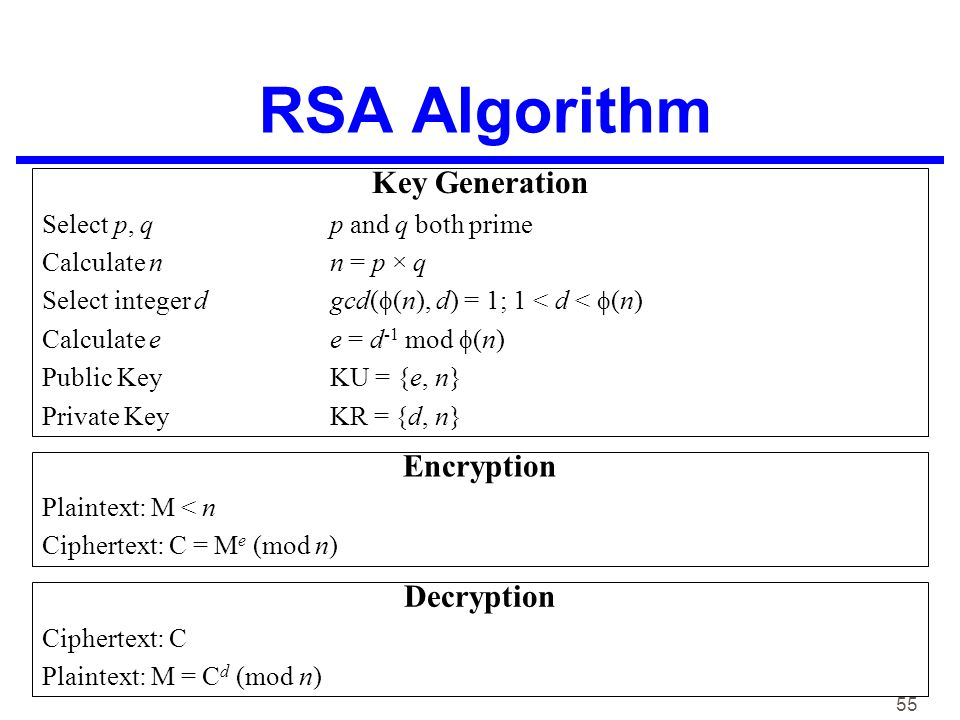
\includegraphics[totalheight=6cm]{rsa.jpg}
%    \caption{}
%    %\label{i}
%\end{figure}

%\begin{figure}
%\centering
%        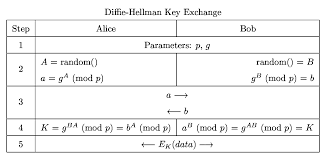
\includegraphics[totalheight=5cm]{dh.png}
%    \caption{}
%    %\label{ii}
%\end{figure}

%\begin{figure}
%\centering
%        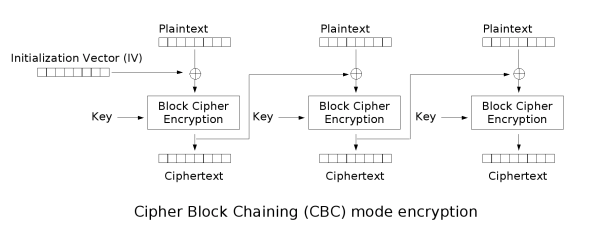
\includegraphics[totalheight=5cm]{Cbc_encryption.png}
%    \caption{}
    %\label{i}
%\end{figure}

\begin{thebibliography}{9}
\bibitem
{LCM} Auguste Kerckhoffs, \emph{La cryptographie militaire}, Journal des sciences militaires, vol. IX, pp. 5–83, January 1883, 161-191.

\bibitem
{PCM} Timothy Gowers (Ed.), June Barrow-Green and Imre Leader (Assoc. Eds.). \emph{The Princeton Companion to Mathematics}. Princeton University Press, Princeton, NJ, 2008, 887-895.

\bibitem
{NDC} Diffie, W., and Hellman, M. \emph{New directions in cryptography}. IEEE Trans. Inform. Theory IT-22, (Nov. 1976), 644-654.

\bibitem
{RSA}Rivest, R.; Shamir, A.; Adleman, L. (February 1978). \emph{A Method for Obtaining Digital Signatures and Public-Key Cryptosystem}, Communications of the ACM. 21 (2): 120-126.


\end{thebibliography}

\end{document}
